% !TeX spellcheck = de_DE/GB

\chapter{Beschreibung der Hardware des Arduino Nano 33 BLE Sense Lite}
\begin{figure}[htb]
	\begin{center}
		
		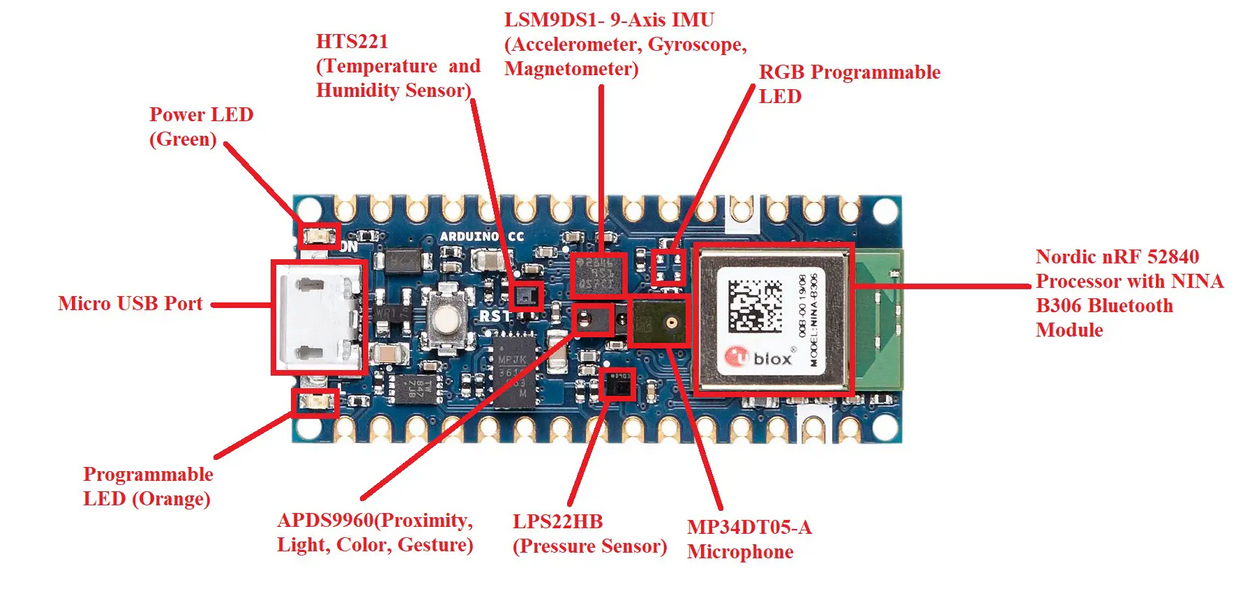
\includegraphics[width=\textwidth]{General/ArduinoBoard.png}
		\caption{Arduino Nano 33 BLE Sense}\cite{eTech.2021} \label{Arduino Nano 33 BLE Sense}
	\end{center}
\end{figure}
\section{Aufbau des Arduinos}
\cite{Ard}
\\
Der Arduino Nano 33 Bluetooth Low Energie (BLE) Sense Lite ist ein Mikrocontroller basierend auf dem Nordic nRF52840-SoC (System-on-a-Chip). Trotz seiner kompakten Bauweise mit einer Größe von 45 x 18 mm verfügt es über mehrere verschiedene integrierte Sensoren, Aktoren und konnektive Schnittstellen (siehe \autoref{Arduino Nano 33 BLE Sense}). Zudem hat der Arduino-Prozessor einen 1 MB Flash-Speicher und 256 KB RAM. Bei dem Prozessor handelt es sich um einen Arm \textregistered Cortex-M4F Prozessorkern, welcher für eingebettete Systeme und Mikrocontroller Anwendungen optimiert ist. Dieser bietet eine gute Leistung bei geringen Stromverbrauch und ist für Echtzeitverarbeitungsaufgaben geeignet. Außerdem besitzt der Prozessor eine Floating Point Unit (FPU), wodurch sich Datenverarbeitungsoperationen effizient verarbeiten lassen.\cite{Arm}
Mithilfe einer integrierten Steckverbindung (engl. \glqq header \grqq) kann der Mikrocontroller direkt auf ein Board gesteckt werden. Zu den integrierten Sensoren, Aktoren und Schnittstellen gehören:
\\ \emph{(Hinweis: Der Arduino Nano 33 BLE Sense Lite ist eine komprimierte Variante vom ursprünglichen Arduino Nano 33 BLE Sense, welcher zusätzlich noch über einen Temperatur- und Feuchtigkeitssensor verfügt!)} 

\begin{itemize}
	\item \textbf{Integrierte Sensoren}: 9-Achsen-IMU (Beschleunigungsmesser, Gyroskop und Magnetometer), Drucksensor, Temperatursensor, Mikrophon und einen Lichtsensor
	\item \textbf{Konnektivität}: Bluetooth Low Energy (BLE), NFC und eine USB-Schnittstelle
	\item \textbf{Stromversorgung}: Über USB oder dem Voltage Input (VIN) -Pin
	\item \textbf{Anschlüsse}: 14 digitale Pins (D2-D12 mit Pulsweitenmodulation), 8 analoge Eingänge (A0-A7 mit Pulsweitenmodulation) 
	\item  \textbf{4 LED-Lampen}: 
	\subitem Power-LED (grün): Zeigt an, dass das Arduino-Board eingeschaltet ist.
	\subitem Programmierbare LED (orange)
	\subitem Programmierbare RGB-LED
\end{itemize}

\section{Integrierte Sensorik}
Der Arduino Nano 33 BLE-Sense Lite verfügt über eine Vielzahl von integrierten Sensoren und Aktoren mit denen verschiedene Umwelteigenschaften detektiert werden können. Zu diesen Sensoren gehören:
\subsection{9-Achs-IMU für die Bewegungserkennung (LSM9DS1)}
	Die Trägheitsmesseinheit LSM9DS1 ist ein System-in-Package, d.h. auf engsten Raum werden mehrere elektronische Komponenten oder Chips in einem Paket miteinander kombiniert.\cite{Wag} Die IMU verfügt über einen 3D-Linearbeschleunigungsmesser, ein 3D-Gyroskop und einen 3D Magnetometer. Außerdem beinhaltet das System eine serielle I2C-Bus Schnittstelle, die einen Standard und einen Fast Mode (100/400 kHz) bereitstellt außerdem eine serielle SPI-Standardschnittstelle. Der Sensor hat einen linearen Beschleunigungsmesser (Accelerometer) mit wählbarer Skala von ±2g/±4g/±8/±16 g, es misst die lineare Beschleunigung in drei Achsen (x, y, z) und ermöglicht die Erfassung von Änderungen der Geschwindigkeit und Position. Das Magnetfeld ist mit einer wählbaren Skala von ±4/±8/±12/±16 Gauß ausgestattet, damit misst es das magnetische Feld in den drei Achsen und ermöglicht die Bestimmung der Ausrichtung relativ zur Erdmagnetfeldrichtung. Das 3D-Gyroskop ist mit wählbarem Skalenendwert: ±125/±250/±500/±1000/±2000 $\frac{Grad}{s}$ und ist dafür zuständig, die Winkelgeschwindigkeit bzw. Drehbewegung um die drei Achsen zu erfassen.\cite{STM1}
	Mögliche Anwendungsbereiche sind zum Beispiel eine Bewegungssteuerungen (Drohnensteuerung, Robotik und industrielle Automatisierung), Schwingungsüberwachung und -kompensation, Antennen, Plattformen, optische Bild- und Objektivstabilisierung.  
\subsection{Näherungs-,Umgebungslicht-, Farb- und Gestensensor (APDS9960)}
	Hierbei handelt sich um einen sehr vielseitigen Sensor. Er dient zur Gestenerkennung, Farberkennung, Abstandsmessung und Umgebungslichtmessung. Die Gestenerkennung nutzt vier gerichtete Fotodioden, um reflektierte Infrarot-Energie (die von der integrierten LED stammt) zu erfassen, um die physischen Bewegungsinformationen (d.h. Geschwindigkeit, Richtung und Entfernung) in digitale Informationen zu übersetzen. Die Näherungserkennung ermöglicht die Messung der Entfernung, durch die Erkennung der reflektierten Infrarot-Energie, (von der integrierten LED) mit Hilfe einer Fotodiode. Erkennungsereignisse sind interruptgesteuert und treten immer dann auf, wenn das Näherungsergebnis die oberen und/oder unteren Schwellenwerte überschreitet. Der Sensor verfügt zudem über Offset-Einstellregister, um den System-Offset zu kompensieren, der durch unerwünschte Infrarot-Energiereflexionen am Sensor entsteht. Die Infrarot-LED-Intensität ist werksseitig eingestellt, so dass eine Kalibrierung der Endgeräte aufgrund von Bauteilschwankungen nicht erforderlich ist.	Die Farb- und Umgebungslichterkennung liefert Daten zur roten, grünen, blauen Farbspektrum und Daten zur klaren Lichtintensität. Jeder der Kanäle R, G, B, C hat einen UV- und Infrarot-Sperrfilter und einen speziellen Datenkonverter, der gleichzeitig 16-Bit-Daten erzeugt. Diese Architektur ermöglicht Anwendungen eine genaue Messung des Umgebungslichts zu messen und die Farbe zu erkennen, was es den Geräten wiederum ermöglicht, die Farbtemperatur zu berechnen und die Hintergrundbeleuchtung des Displays dementsprechend anzupassen.\cite{AT}
\subsection{Barometrischer Drucksensor (LPS22HB)}
	Der LPS22HB ist ein sehr kompakter Absolutdrucksensor, der auf dem piezoresistiven Prinzip basiert. Er fungiert als Barometer und verfügt über einen digitalen Ausgang. Das Gerät besteht aus einem Sensorelement und einer Integrated-Circuit (IC)-Schnittstelle, die eine Kommunikation zwischen der Sensoreinheit und der Anwendung über Inter-Integrated Circuit (I2C) oder Serial Peripheral Interface (SPI) ermöglicht. Das Sensorelement erfasst den absoluten Druck und besteht aus einer speziell hergestellten, aufgehängten Membran. Der LPS22HB ist in einem vollständig vergossenem Land Grid Array (LGA) -Gehäuse untergebracht, das kleine Löcher aufweist. Durch diese Öffnung gelangt der externe Druck auf das Sensorelement. Der Betrieb des Sensors ist über einen Temperaturbereich von -40 °C bis +85 °C gewährleistet.\cite{STM2}
	Anwendungsbereiche für diesen Sensor währen zum Beispiel: Wetterstationen, Höhenmesser, Luftdrucküberwachung in industriellen Prozessen oder tragbare smarte Geräte, wie Sportuhren oder Smartphones.
\subsection{Digitales Mikrophon (MP34DT05)}
	Das MP34DT05-A ist ein kleines, energiesparendes Mikrophon mit kapazitiven Sensor. Es verwendet ein spezielles Silizium-Mikrobearbeitungsverfahren, um Schallsignale zu erkennen. Das Mikrofon hat eine Schnittstelle, die ein digitales Signal in einem speziellen Format bereitstellen kann. Darüber hinaus ist es ein hochwertiges Mikrofon mit geringer Verzerrung, gutem Signal-Rausch-Abstand von 64 dB und hoher Empfindlichkeit von -26 dBFS ±3 dB. Es ist in einem kompakten Gehäuse erhältlich und funktioniert bei Temperaturen im Bereich von -40 °C bis +85 °C. Abmessungen des Gehäuses HCLGA-4 LD sind 3 x 4 x 1 (in mm).\cite{StmicElec.2021}

\section{Beschreibung der Schnittstellen}
Der Arduino Nano 33 BLE-Sense bietet eine Vielzahl von Schnittstellen, die das Board mit anderen Komponenten und Geräten einfach verbinden lassen. Hier sind einige Details zu den wichtigsten Schnittstellen des Boards:
\bigskip
\begin{figure}[htb]
	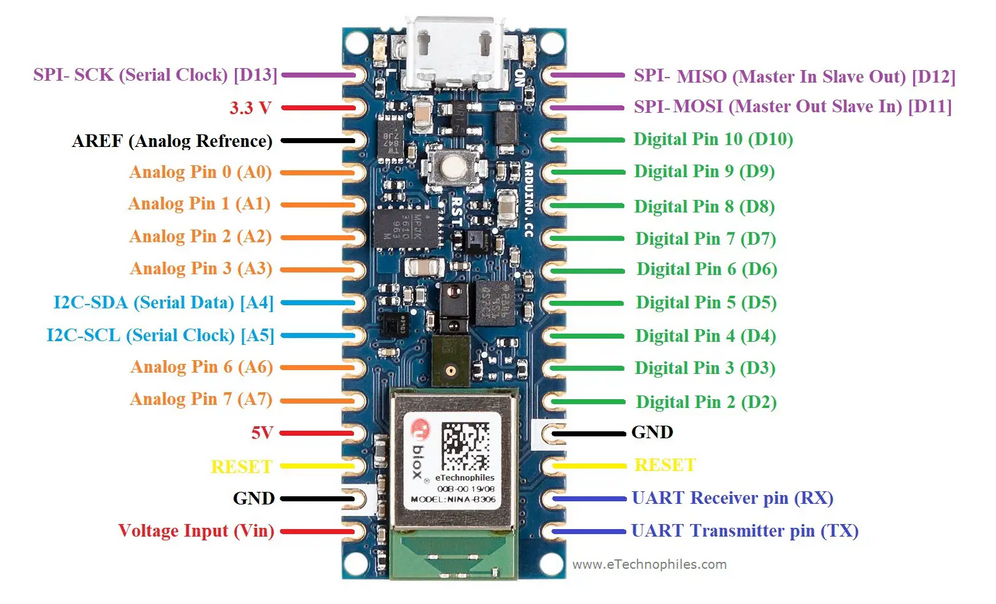
\includegraphics[width=14cm]{General/ArduinoPinBoard.png}
	\caption{Arduino Nano Pinboard} \label{Arduino Nano Pinbout}\begin{center}
		\cite{Arduino2023}
	\end{center}
\end{figure}

\section{Digitale Ein- und Ausgangspins}

Das Board verfügt über 14 digitale Ein- und Ausgangspins, Die digitalen Arduino-Pins können nur zwei Zustände lesen: wenn ein Spannungssignal vorliegt und wenn kein Signal vorhanden ist. Diese Art der Eingabe wird normalerweise als digital (oder binär) bezeichnet, und diese Zustände werden als HIGH und LOW oder 1 und 0 bezeichnet.
Alle digitalen Pins mit den Nummern D0 bis D13 sind PWM-fähige Pins, was bedeutet, dass sie in der Lage sind, ein Pulsweitenmodulationssignal mit einer Auflösung von 8 Bit zu erzeugen. Mit der Funktion analogWrite() kann ein PWM-Signal auf diesen Pins erzeugt werden.\cite{eTech.2021}\cite{ArdSense.2023}

\subsection{Analoge Eingangspins:}
Die Platine hat zusätzlich 8 analogen Eingangspins (A0 bis A7), diese analogen Ausgänge können nur über PWM-Pins erreicht werden. Das bedeutet, dass wir bis zu 8 analoge Eingangssensoren an die Platine anschließen können. Die Funktion von analogen Pins besteht darin, den Wert der analogen Sensoren zu lesen, die in der Schaltung verwendet werden. Jeder dieser analogen Pins verfügt über einen eingebauten ADC mit einer Auflösung von 212 Bits.

\subsection{UART:}
Das Board hat eine UART-Schnittstelle, die für die serielle Kommunikation mit anderen Geräten oder Mikrocontrollern verwendet werden kann. Diese Schnittstelle verwendet die Pins D0 und D1.

\subsection{I2C:}
Die Platine verfügt über eine I2C-Schnittstelle, die zur Kommunikation mit verschiedenen Geräten wie Sensoren und Displays verwendet werden kann. Diese Schnittstelle nutzt die Pins A4 und A5. Das I2C-Protokoll ist ein serieller Zweidraht-Kommunikationsstandard, steht für Inter-Integrated Circuits. Zur Übertragung von Daten werden zwei Pins verwendet: ein serieller Uhren-pin (SCL) und ein serieller Daten-pin (SDA). Der SCL-Pin (Serial Clock) überträgt die Taktdaten und synchronisiert die Übertragung von Daten zwischen den beiden Geräten. Der Master-Gerät generiert die serielle Uhr. Der SDA-Pin (Serial Data) dient als Datenleitung, die von Slave- und Master-Geräten zum Senden und Empfangen von Daten verwendet werden. Im Gegensatz dazu wird der SCL als Taktleitung bezeichnet. Die I2C-Pins auf der Platine sind A4 (SDA) und A5 (SCL). 
\subsection{PI:}
Das Akronym SPI steht für Serial Peripheral Interface. Dieses Protokoll wird von Mikrocontrollern genutzt, um eine schnelle Kommunikation mit einem oder mehreren Peripheriegeräten zu ermöglichen. Es gibt drei gemeinsame Pins für alle Peripheriegeräte:
\begin{itemize}
	\item SCK: Dies steht für Serial Clock und erzeugt Taktimpulse zur Synchronisation der Datenübertragung.
	\item MISO: Dies steht für Master Input/Slave Output und wird genutzt, um Daten an den Master zu senden.
	\item MOSI: Dies steht für Master Output/Slave Input und wird genutzt, um Daten an die Slaves/Peripheriegeräte zu senden.
\end{itemize}
Die SPI-Pins auf der Platine sind D13 (SCK), D12 (MISO) und D11 (MOSI). RXD und TXD werden für die serielle Kommunikation genutzt. Der TXD-Pin wird zur Übertragung von Daten genutzt. Die RXD-Pin für den Empfang von Daten, während der seriellen Kommunikation. Die Pins stellen auch den erfolgreichen Datenfluss vom Computer zur Platine her. Die UART-Pins auf der Platine sind D0 (TX) und D1 (RX).
\\
\subsection{USB:}
Das Board kann über einen Micro-USB Anschluss mit einem Computer verbunden werden, um es zu programmieren oder Daten zu übertragen.
\subsection{Andere Pins:}
\begin{itemize}
	\item \textbf{3,3 V}: Der 3,3-V-Pin arbeitet als geregelte Ausgangsspannung von 3,3 V.
	\item \textbf{5V}: Der 5V-Pin gibt 5V an die externen Komponenten ab. Die Stromquelle von 5 V für das Arduino Nano-Board erfolgt über den USB-Anschluss und den Vin-Pin. 
	\item \textbf{RST-Pin}: Wird genutzt, um eine Reset-Taste zur Verbindung hinzuzufügen, mit der der Mikrocontroller zurückgesetzt werden kann.
	\item \textbf{AREF-Pin}: Der AREF-PIN (analoge Referenz), liefert die Spannungsreferenz, die der Mikrocontroller zur Zeit verwendet. Das Senden eines Signals an diesen Pin hat keinen Effekt. 
\end{itemize}
\section{Beschreibung der Firmware}
Die Firmware des Arduino ist eine spezielle Software, die fest im elektronischen Gerät implementiert und eng mit der Hardware verbunden ist. Im Gegensatz zur klassischen Software ist es untrennbar mit der Hardware verbunden und kann in der Regel nicht einfach vom Benutzer ausgetauscht werden. Firmware wird häufig auf Flash-Speicher, ROM, EPROM oder EEPROM gespeichert. Allgemein ist die Firmware ein wichtiger Bestandteil von elektronischen Geräten, da sie die Funktionen der Hardware steuert und die Interaktion zwischen Hardware und Software erleichtert.Einige der wichtigsten Funktionen der Firmware des Arduino Nano 33 BLE-Sense sind:
\\ \cite{Bruhlmann.2012}
\begin{itemize}
	\item \textbf{Fehlerbehebung}: Firmware enthält Diagnose- und Fehlerbehebungsfunktionen, die dazu beitragen, Probleme zu erkennen und beheben, die in der Hardware auftreten können. Diese Funktionen sind wichtig, um sicherzustellen, dass das Gerät ordnungsgemäß funktioniert und dass Probleme schnell behoben werden können. 
	\item \textbf{Aktualisierung}: Firmware kann aktualisiert werden, um neue Funktionen hinzuzufügen oder bestehende zu verbessern. Die Aktualisierung kann auch dazu beitragen, Sicherheitsprobleme zu Beheben und die Leistung des Gerätes zu verbessern. 
	\item \textbf{Kommunikation}: Die Firmware kann die Kommunikation zwischen verschiedenen Geräten erleichtern, indem sie die Protokolle und Standards implementiert, die für die Kommunikation erforderlich sind.
\end{itemize}
\section{Bezugsquellen}
Für die Beschreibung der Hardware des Arduino Nano 33 wurde sorgfältig recherchiert und auf mehrere zuverlässige Bezugsquellen zurückgegriffen. Diese Quellen umfassten offizielle Datenblätter des Herstellers, um detaillierte technische Informationen über die Komponenten des Arduino Nano 33 zu erhalten. Denn jede Komponente und jeder Sensor ist mit einer eindeutigen Kennzeichnung versehen, die zur Identifikation und zum Auffinden der entsprechenden Datenblätter dient. Diese Datenblätter bieten eine umfassende Dokumentation über die Spezifikationen, Funktionen und Eigenschaften der Hardwarekomponenten.



